\documentclass[10pt,a4paper]{article}
\usepackage{a4wide}
\usepackage[utf8]{inputenc}
\usepackage[slovene]{babel}% You have to adjust the language here 
\usepackage[T1]{fontenc}
\usepackage{epsfig}
\usepackage{subfigure}
\usepackage{fancyhdr} %package for header design
\usepackage{color}
\usepackage{hyperref}
\hypersetup{
    colorlinks=true,
    linkcolor=blue,
    filecolor=magenta,      
    urlcolor=blue,
}
\usepackage{graphicx}

%packages for symbols 
\usepackage{ifsym}

%mathematic package
\usepackage{amsmath}
 
%package for tables. Table generator in on webpage: https://www.tablesgenerator.com/
\usepackage[table,xcdraw]{xcolor}

%packages for design and align picture on coverpage
\usepackage{chngpage} 
\usepackage{calc}

%packages for configure own listings
\usepackage{listings,xcolor}

\usepackage{textgreek}

%definitions of BASCOM code colors
\definecolor{blue_keywords}{rgb}{0,0,0.5}
\definecolor{green_comments}{rgb}{0,0.5,0}
\definecolor{turqusnumbers}{rgb}{0.17,0.57,0.69}
\definecolor{teal_strings}{rgb}{0,0.5,0.5}
\definecolor{maroon_HW_register}{rgb}{0.5, 0, 0}
\definecolor{bg_gray}{rgb}{0.9, 0.9, 0.9}
\definecolor{fuchsia_user_function}{rgb}{1, 0, 0.5}
\definecolor{ASM_purple}{RGB}{128, 0, 128}

%https://tex.stackexchange.com/questions/235731/listings-syntax-for-literate
%https://tex.stackexchange.com/questions/172945/coloring-in-listing

%setting for BASCOM code (keywords)- function for include .bas file
\lstdefinelanguage{bascom}
{keywords=[1]{regfile, crystal, include, do, loop, end, while, wend, for, next, dim, as, output, input, alias, waitms, wait, waitus, print, cls, lcd, noblink, config, initlcd, include, return, locate, gosub, goto, function, declare, sub, if, then, else, elseif, end if, getadc, fusing, chr, as, string, word, single, integer, byte, bit, baud, Enable, Interrupts, start, stop, cursor, off, shift, left, right, asm, Open, Close, Binary, hex, bin, I2cstart, I2cwbyte, err, I2cstop, I2cinit, lib, step, hwstack , swstack, framesize, at, overlay, i2crbyte, ack, nack, nop, select, case, low, high, inkey, lowerline, printbin, version, noecho, instr, mid, len, debounce, toggle, const, load, on, timer, bitwait, reset, to, not }, %BASCOM key words
    keywordstyle=[1]\color{blue_keywords},
    keywords=[2]{pwm0b, pwm0a,Pwm1a, Pwm1b, Pwm2a, Pwm2b, PORTB, PORTC, PORTD, PORTA, PINA, PINB, PINC, PIND, PIN, PORT, Nvm_cmd, Cpu_ccp, Rampz, _romsize, NVM_STATUS, Timer1, Timer0, Timer2, Ocr1a, Ocr1b, twbr, twsr},
    keywordstyle=[2]\color{maroon_HW_register},%registers and other key words 
	keywords=[3]{izmeriuz_mm, Rx_data, Poweronsim, Poweroffsim, preveriomrezje, Potrdi, send_CMD, Status, Flushbuf, Getline, Showsms, motor3, motor2, motor1},%own functions    
    keywordstyle=[3]\color{fuchsia_user_function},
    keywords=[4]{Ldi, st, LDS, SBRC, RJMP RAMPZ, rjmp, sts, spm},    
    keywordstyle=[4]\color{ASM_purple},
    sensitive=false,
    morecomment=[l][\color{green_comments}]{'},
    morestring=[b]",
    stringstyle=\color{teal_strings},
    showstringspaces=false,
    showspaces=false,
    showtabs=false,
    breaklines=true,                  
    tabsize=2,
    basicstyle=\ttfamily\small,
    backgroundcolor=\color{bg_gray},
    breaklines=true,
    columns=fullflexible,
    frame=single,
    numbers=left,
    numbersep=5pt,
    title=\lstname,
    numberstyle=\tiny\color{gray},
    literate=*
    	{=}{{\textcolor{red}{=}}}1
    	{ ; }{{\textcolor{red}{ ; }}}1
    	{ , }{{\textcolor{red}{ , }}}1
    	{(}{{\textcolor{red}{(}}}1
        {*}{{\textcolor{red}{*}}}1
        {+}{{\textcolor{red}{+}}}1
        {-}{{\textcolor{red}{-}}}1
        {)}{{\textcolor{red}{)}}}{1}
        {:}{\textcolor{red}{:}}{1}
        {\{}{\textcolor{red}{\{}}{1}
        {\}}{\textcolor{red}{\}}}{1}
        {<}{\textcolor{red}{<}}{1}
        {>}{\textcolor{red}{>}}{1}
        {\&}{\textcolor{red}{\&}}{1}
        {\#}{\textcolor{red}{\#}}{1}
        {!}{\textcolor{ASM_purple}{!}}{1}
        {\$}{{\textcolor{blue_keywords}{\$}}}{1}%
    }
%function for writing BASCOM code directly
\lstnewenvironment{Bascomlisting}
  {
    \lstset{
        language=bascom,
        basicstyle=\ttfamily \small,
        breaklines=true,
        columns=fullflexible,
        backgroundcolor=\color{bg_gray},
        frame=single,
        numbers=left,
        numbersep=5pt,
        numberstyle=\tiny\color{gray},}
  }
  {%important
  }%important
\lstset{language=bascom}

%this code is for red brackets
\usepackage{etoolbox} % provides the \patchcmd macro
\makeatletter
\patchcmd{\lsthk@SelectCharTable}{`)}{``}{}{} % patch listings
%\patchcmd{\lsthk@SelectCharTable}{``}{`)}{}{} % undo patch if needed
\makeatother
%end code for red brackets

%package fot todo notes
\usepackage[colorinlistoftodos,prependcaption]{todonotes}
\usepackage{epsfig} %%package for including picrures 

\begin{document}
\baselineskip 19pt \thispagestyle{empty}

%%*
\begin{center}
{\Huge\bf \LaTeX\ template for BASCOM code}\\
[1cm] {\large \bf Template for writing BASCOM code in \LaTeX\ }\\


Avthor: Tomaž Kušar

november, 2019\linebreak 
\begin{figure}[h!] %\centering
\begin{adjustwidth}{-\oddsidemargin-1in}{-\rightmargin}
 
\includegraphics[width=210mm]{./images/BASCOM_start.png}\\
%\epsfig{file=slike/naslovna.jpg,angle=0, width=\paperwidth}
\end{adjustwidth}
\end{figure}

\end{center}
%\newpage
\clearpage \setcounter{page}{2}
\newpage

%\noindent \textbf{Read me}\\

%\newpage

%\tableofcontents
\newpage
\pagestyle{fancy}
\renewcommand{\sectionmark}[1]{\markright{Template for BASCOM code }}
\renewcommand{\subsectionmark}[1]{\markright{Template for BASCOM code}}
\renewcommand{\subsubsectionmark}[1]{\markright{Template for BASCOM code}}


\section{About template}
The template is intended for writing documents containing BASCOM code and shows how to write BASCOM code directly with a \LaTeX\  program, or by including a .bas file directly in a document.  The template is very useful for writing documentation.

All BASCOM keywords are colored blue, red, green, purple...

This way of writing is very fast. The BASCOM code is colored and transparent and there is no need to deal with any document formatting.

\section{Quick start}
For quick start, follow this steps:
\begin{itemize}
\setlength{\itemsep}{0pt}%
\setlength{\parskip}{0pt}%
\item Install Ghostscripts (\href{https://www.ghostscript.com/download.html} {https://www.ghostscript.com/download.html})
\item Install MiKTeX on computer from site \href{https://miktex.org/download}{https://miktex.org/download}. 
\item This template is written with Texmaker editor. You can download it from site\\ \href{https://www.xm1math.net/texmaker/}{https://www.xm1math.net/texmaker/}.
\item Open \texttt{template\_BASCOM-code.tex} file in Texmaker and compile it.
\end{itemize}

\todo[inline]{NOTE: This template is \textbf{beta version} and doesen't include all bascom keywords yet. You can add keywords into preamble of template by yourself. }
\section{Corrections in version 2}
\begin{itemize}
\setlength{\itemsep}{0pt}%
\setlength{\parskip}{0pt}%
\item New keywords
\item Properly colored brackets
\begin{Bascomlisting}
Dim answer(10) As String * 60
Getadc(3) 
\end{Bascomlisting}
\end{itemize}

\newpage
\section{Including .bas file}
\lstinputlisting[language=bascom]{bascom/led_on_off.bas}

\newpage
\section{Example included asm code}
\lstinputlisting[language=bascom]{bascom/asm_code_template.bas}
\newpage
\section{Write BASCOM code directly into document}
You could include BASCOM code into document by copying text directly:

\begin{Bascomlisting}
'input button example
$regfile = "m328pdef.dat"
$crystal = 16000000

Config Portb = Output
Config Portc = Input
'config pull-up
Portc = 63

Do
   If Pinc.1 = 0 Then
      Portb.5 = 1
   Else
      Portb.5 = 0
   End If
Loop

End
\end{Bascomlisting}
\newpage
\section{Example included picture}
\begin{figure}[h!] \centering
 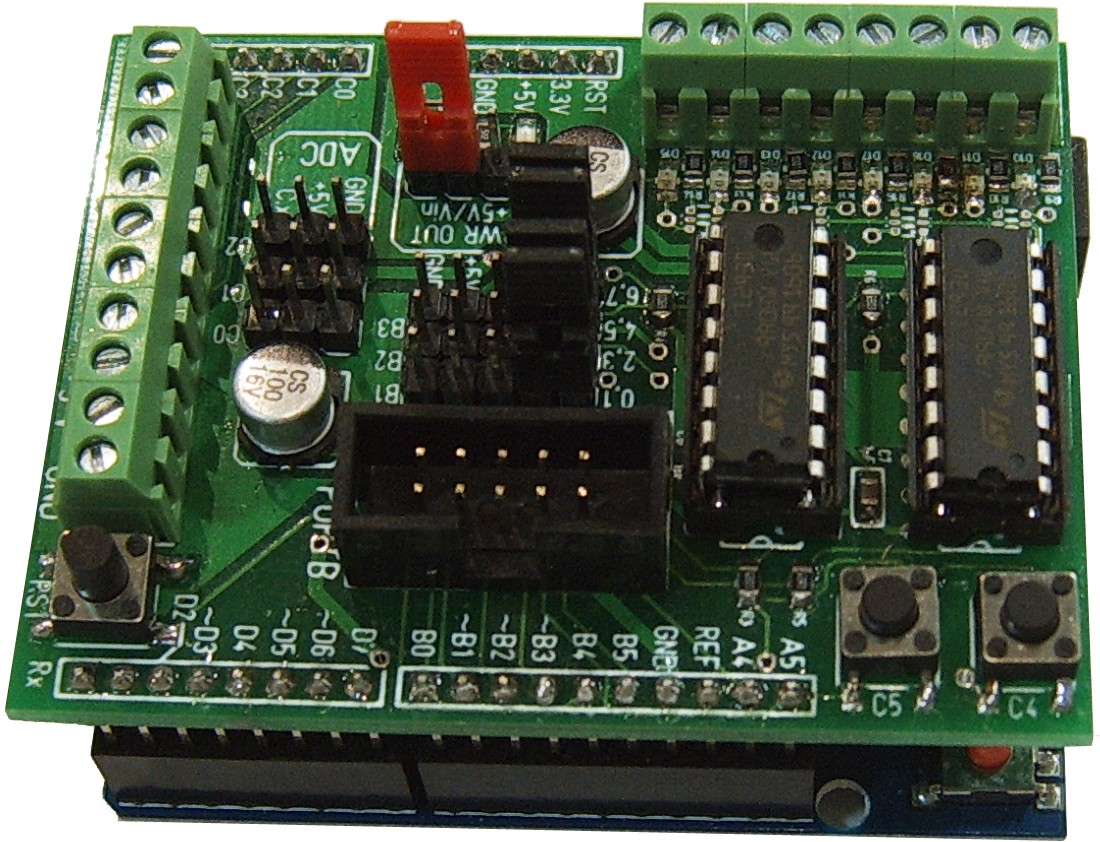
\includegraphics[width=8cm]{pictures/RobDuino.png}
 \caption{Interface RobDuino}
  \label{slika:robduino}
\end{figure}
\newpage
\section{BASCOM code presented in two ways.}
Directly written BASCOM code into this document. 
\begin{Bascomlisting}
'-------------------------------------------------------------------------------
'                ARDUINO-UNO-REV3.BAS
'              (c) 1995-2020, MCS Electronics
'  This is a sample file for the Mega328 based ARDUINO board UNO REV3
'  Select Programmer 'ARDUINO' , 115200 baud and the proper COM port
'-------------------------------------------------------------------------------
$regfile = "m328def.dat"                                    ' used micro
$crystal = 16000000                                         ' used xtal
$baud = 19200                                               ' baud rate we want
$hwstack = 40
$swstack = 40
$framesize = 40

Config Clockdiv = 1                                         ' either use this or change the divider fuse byte
'-------------------------------------------------------------------------------

Config Portb = Output                                       ' make portb an output
Do
  Toggle Portb                                              ' toggle level
  Waitms 1000                                               ' wait 1 sec
  Print "UNO REV3"                                          ' test serial com
Loop
\end{Bascomlisting}

And included .BAS file. The result is the same.

\lstinputlisting[language=bascom]{bascom/ArduinoUno.bas}




\end{document}



